%%%%%%%%%%%%%%%%%%%%%%%%%%%%%%%%%%%%%%%%%
% Wenneker Article
% LaTeX Template
% Version 2.0 (28/2/17)
%
% This template was downloaded from:
% http://www.LaTeXTemplates.com
%
% Authors:
% Vel (vel@LaTeXTemplates.com)
% Frits Wenneker
%
% License:
% CC BY-NC-SA 3.0 (http://creativecommons.org/licenses/by-nc-sa/3.0/)
%
%%%%%%%%%%%%%%%%%%%%%%%%%%%%%%%%%%%%%%%%%

%----------------------------------------------------------------------------------------
%	PACKAGES AND OTHER DOCUMENT CONFIGURATIONS
%----------------------------------------------------------------------------------------

\documentclass[10pt, a4paper, twocolumn]{article} % 10pt font size (11 and 12 also possible), A4 paper (letterpaper for US letter) and two column layout (remove for one column)



%%%%%%%%%%%%%%%%%%%%%%%%%%%%%%%%%%%%%%%%%
% Wenneker Article
% Structure Specification File
% Version 1.0 (28/2/17)
%
% This file originates from:
% http://www.LaTeXTemplates.com
%
% Authors:
% Frits Wenneker
% Vel (vel@LaTeXTemplates.com)
%
% License:
% CC BY-NC-SA 3.0 (http://creativecommons.org/licenses/by-nc-sa/3.0/)
%
%%%%%%%%%%%%%%%%%%%%%%%%%%%%%%%%%%%%%%%%%

%----------------------------------------------------------------------------------------
%	PACKAGES AND OTHER DOCUMENT CONFIGURATIONS
%----------------------------------------------------------------------------------------

\usepackage[english]{babel} % English language hyphenation

\usepackage{microtype} % Better typography

\usepackage{amsmath,amsfonts,amsthm} % Math packages for equations

\usepackage[svgnames]{xcolor} % Enabling colors by their 'svgnames'

\usepackage[hang, small, labelfont=bf, up, textfont=it]{caption} % Custom captions under/above tables and figures

\usepackage{booktabs} % Horizontal rules in tables

\usepackage{lastpage} % Used to determine the number of pages in the document (for "Page X of Total")

\usepackage{graphicx} % Required for adding images

\usepackage{enumitem} % Required for customising lists
\setlist{noitemsep} % Remove spacing between bullet/numbered list elements

\usepackage{sectsty} % Enables custom section titles
\allsectionsfont{\usefont{OT1}{phv}{b}{n}} % Change the font of all section commands (Helvetica)

%----------------------------------------------------------------------------------------
%	MARGINS AND SPACING
%----------------------------------------------------------------------------------------

\usepackage{geometry} % Required for adjusting page dimensions

\geometry{
	top=1cm, % Top margin
	bottom=1.5cm, % Bottom margin
	left=2cm, % Left margin
	right=2cm, % Right margin
	includehead, % Include space for a header
	includefoot, % Include space for a footer
	%showframe, % Uncomment to show how the type block is set on the page
}

\setlength{\columnsep}{7mm} % Column separation width

%----------------------------------------------------------------------------------------
%	FONTS
%----------------------------------------------------------------------------------------

\usepackage[T1]{fontenc} % Output font encoding for international characters
\usepackage[utf8]{inputenc} % Required for inputting international characters

\usepackage{XCharter} % Use the XCharter font

%----------------------------------------------------------------------------------------
%	HEADERS AND FOOTERS
%----------------------------------------------------------------------------------------

\usepackage{fancyhdr} % Needed to define custom headers/footers
\pagestyle{fancy} % Enables the custom headers/footers

\renewcommand{\headrulewidth}{0.0pt} % No header rule
\renewcommand{\footrulewidth}{0.4pt} % Thin footer rule

\renewcommand{\sectionmark}[1]{\markboth{#1}{}} % Removes the section number from the header when \leftmark is used

%\nouppercase\leftmark % Add this to one of the lines below if you want a section title in the header/footer

% Headers
\lhead{} % Left header
\chead{\textit{\thetitle}} % Center header - currently printing the article title
\rhead{} % Right header

% Footers
\lfoot{} % Left footer
\cfoot{} % Center footer
\rfoot{\footnotesize Page \thepage\ of \pageref{LastPage}} % Right footer, "Page 1 of 2"

\fancypagestyle{firstpage}{ % Page style for the first page with the title
	\fancyhf{}
	\renewcommand{\footrulewidth}{0pt} % Suppress footer rule
}

%----------------------------------------------------------------------------------------
%	TITLE SECTION
%----------------------------------------------------------------------------------------

\newcommand{\authorstyle}[1]{{\large\usefont{OT1}{phv}{b}{n}\color{DarkRed}#1}} % Authors style (Helvetica)

\newcommand{\institution}[1]{{\footnotesize\usefont{OT1}{phv}{m}{sl}\color{Black}#1}} % Institutions style (Helvetica)

\usepackage{titling} % Allows custom title configuration

\newcommand{\HorRule}{\color{DarkGoldenrod}\rule{\linewidth}{1pt}} % Defines the gold horizontal rule around the title

\pretitle{
	\vspace{-30pt} % Move the entire title section up
	\HorRule\vspace{10pt} % Horizontal rule before the title
	\fontsize{32}{36}\usefont{OT1}{phv}{b}{n}\selectfont % Helvetica
	\color{DarkRed} % Text colour for the title and author(s)
}

\posttitle{\par\vskip 15pt} % Whitespace under the title

\preauthor{} % Anything that will appear before \author is printed

\postauthor{ % Anything that will appear after \author is printed
	\vspace{10pt} % Space before the rule
	\par\HorRule % Horizontal rule after the title
	\vspace{20pt} % Space after the title section
}

%----------------------------------------------------------------------------------------
%	ABSTRACT
%----------------------------------------------------------------------------------------

\usepackage{lettrine} % Package to accentuate the first letter of the text (lettrine)
\usepackage{fix-cm}	% Fixes the height of the lettrine

\newcommand{\initial}[1]{ % Defines the command and style for the lettrine
	\lettrine[lines=3,findent=4pt,nindent=0pt]{% Lettrine takes up 3 lines, the text to the right of it is indented 4pt and further indenting of lines 2+ is stopped
		\color{DarkGoldenrod}% Lettrine colour
		{#1}% The letter
	}{}%
}

\usepackage{xstring} % Required for string manipulation

\newcommand{\lettrineabstract}[1]{
	\StrLeft{#1}{1}[\firstletter] % Capture the first letter of the abstract for the lettrine
	\initial{\firstletter}\textbf{\StrGobbleLeft{#1}{1}} % Print the abstract with the first letter as a lettrine and the rest in bold
}

%----------------------------------------------------------------------------------------
%	BIBLIOGRAPHY
%----------------------------------------------------------------------------------------

\usepackage[backend=bibtex,style=authoryear,natbib=true]{biblatex} % Use the bibtex backend with the authoryear citation style (which resembles APA)

\addbibresource{example.bib} % The filename of the bibliography

\usepackage[autostyle=true]{csquotes} % Required to generate language-dependent quotes in the bibliography
 % Specifies the document structure and loads requires packages
\setlength{\parskip}{1em}
\setlength\parindent{0pt}

%----------------------------------------------------------------------------------------
%	ARTICLE INFORMATION
%----------------------------------------------------------------------------------------

\title{Reconnaissance de dessins manuscrits: projet end-to-end} % The article title

\author{
	\authorstyle{William Bourget et Samuel Lévesque} % Authors
	\newline\newline % Space before institutions
	\institution{Département d'informatique et de génie logiciel \\Université Laval, Québec, Qc, Canada\\} % Institution 1
	%\textsuperscript{2}\institution{University of Texas at Austin, Texas, United States of America}\\ % Institution 2
	%\textsuperscript{3}\institution{\texttt{LaTeXTemplates.com}} % Institution 3
}

% Example of a one line author/institution relationship
%\author{\newauthor{John Marston} \newinstitution{Universidad Nacional Autónoma de México, Mexico City, Mexico}}

\date{10 mai 2019} % Add a date here if you would like one to appear underneath the title block, use \today for the current date, leave empty for no date

%----------------------------------------------------------------------------------------

\begin{document}

\maketitle % Print the title

\thispagestyle{firstpage} % Apply the page style for the first page (no headers and footers)

%----------------------------------------------------------------------------------------
%	ABSTRACT
%----------------------------------------------------------------------------------------

On souhaite réaliser un projet \emph{end-to-end} en traitement d'images pour couvrir toutes les étapes d'un projet en analyse prédictive tout en se familiarisant avec les solutions d'infonuagique et de travailler avec des données massives.

En utilisant des transformations de données sur nos intrants vectoriels, on arrive à arrimer notre interface graphique avec nos données d'entraînement. 

Aussi, en utilisant une technique d'échantillonnage ciblé, on obtient des gains de précision de 2\% par rapport à un entraînement standard sur notre architecture \emph{ResNet18}. 

Avec un modèle par ensemble simple et nos deux classificateurs \emph{ResNet18}, on obtient une \emph{Mean Average Precision} sur 3 prédictions de 85.66\% et les prédictions du modèle semblent naturelles pour l'humain même lorsqu'elles ne correpondent pas à l'étiquette réelle de l'image qu'on tente de classifier.

L'utilisation de l'évolution temporelle des dessins et classificateurs moins corrélés et plus spécialisés dans notre modèle par ensemble nous permettrait d'augmenter les performances globales de notre modèle prédictif et de se rapprocher de l'état de l'art qui fournit des performances avoisinants les 95\% en MAP@3.

%----------------------------------------------------------------------------------------
%	ARTICLE CONTENTS
%----------------------------------------------------------------------------------------

\section{Introduction}

C'est l'intro 

das
d
as
da
sd
as
gsd
h
hhhhhhfghfgh tdh fgj fdj fg fg

\section{Description des données}
Google AI rend disponible une partie du jeux de données de \emph{Quick, Draw}\footcite{Qd:Data} qui est constitué de milliards de dessins faits à la main par différents utilisateurs sur leur plateforme web. 


Les données sont fournies sous forme de fichiers csv (1 par classe) contenant principalement des vecteurs de positions du crayon dans le temps ayant permis de réaliser les traits du dessin, le pays de l'utilisateur et la classe du dessin.

Les dessins sont composés de vecteurs distincts représentants chacun des traits de crayon et chaque vecteur est composé de points tridimensionnels (x, y, temps écoulé depuis le premier point du vecteur).
Cette manière de présenter les dessins permet de sauver une grande quantité d'espace mémoire puisque ces données sont beaucoup moins volumineuses que des fichiers d'images brutes.

Il s'agit d'un jeu de données extrêmement volumineux, on note certaines caractéristiques :

\begin{itemize}
	\item \textbf{340 classes} (Types de dessins différents).
	\item \textbf{$\approx$ 150 000 images/classe}.
	\item Plus de \textbf{51 millions d'images} au total
	\item \textbf{24,4 Gb} de données sous format .csv.
\end{itemize}



\section{Contraintes et enjeux}
Une quantité de données aussi importante crée des enjeux et problèmes importants dans l'entraînement du réseau. On présente ici les enjeux principaux qui nous amènent à tester différentes manières d'entraînement.


\subsection{Enjeux de mémoire}

Pour pouvoir utiliser des réseaux de neurones à convolution, il faut utiliser des données étant sous forme d'image. Étant donné la quantité massive de données, il ne semble pas optimal de transformer toutes les données du format csv en images directement avant l'entraînement. Pour pallier à ce problème et pour pouvoir utiliser des réseaux pré-entraîné , on transforme le format csv des traits de crayon au moment où on charge les données dans le modèle.

\subsection{Enjeux de performance}

La quantité massive de données ne nous permet pas de faire des epochs traditionnelles. En effet, avec les moyens de calculs que nous utilisons (\emph{Google Colab}) , une seule epoch peut prendre environ 1 mois en calculant 24h/24.

Pour cette même raison, on ne peut pas tester une grande quantité d'hyperparamètres. Il faut se limiter un ensemble d'hyperparamètres pour chacun des modèles que l'on veut tester.


\subsection{Enjeux d'une application réelle}

La mise en place d'une application concrète nous amène également quelques contraintes supplémentaires. L'application créée nous fait perdre l'information temporelle des traits de crayons puisque la sortie de l'application est une image de format png. On ne peut donc pas utiliser l'ordre dans lequel les traits ont été dessinés par l'utilisateur. Il nous est donc impossible d'utiliser différents canaux pour simuler l'évolution temporelle du dessin







\section{Transformations des données}



La figure \ref{transformationimage} nous montre un exemple de transformation d'une image de maison réalisé en 2 traits de crayons. 

\begin{figure}[h]
	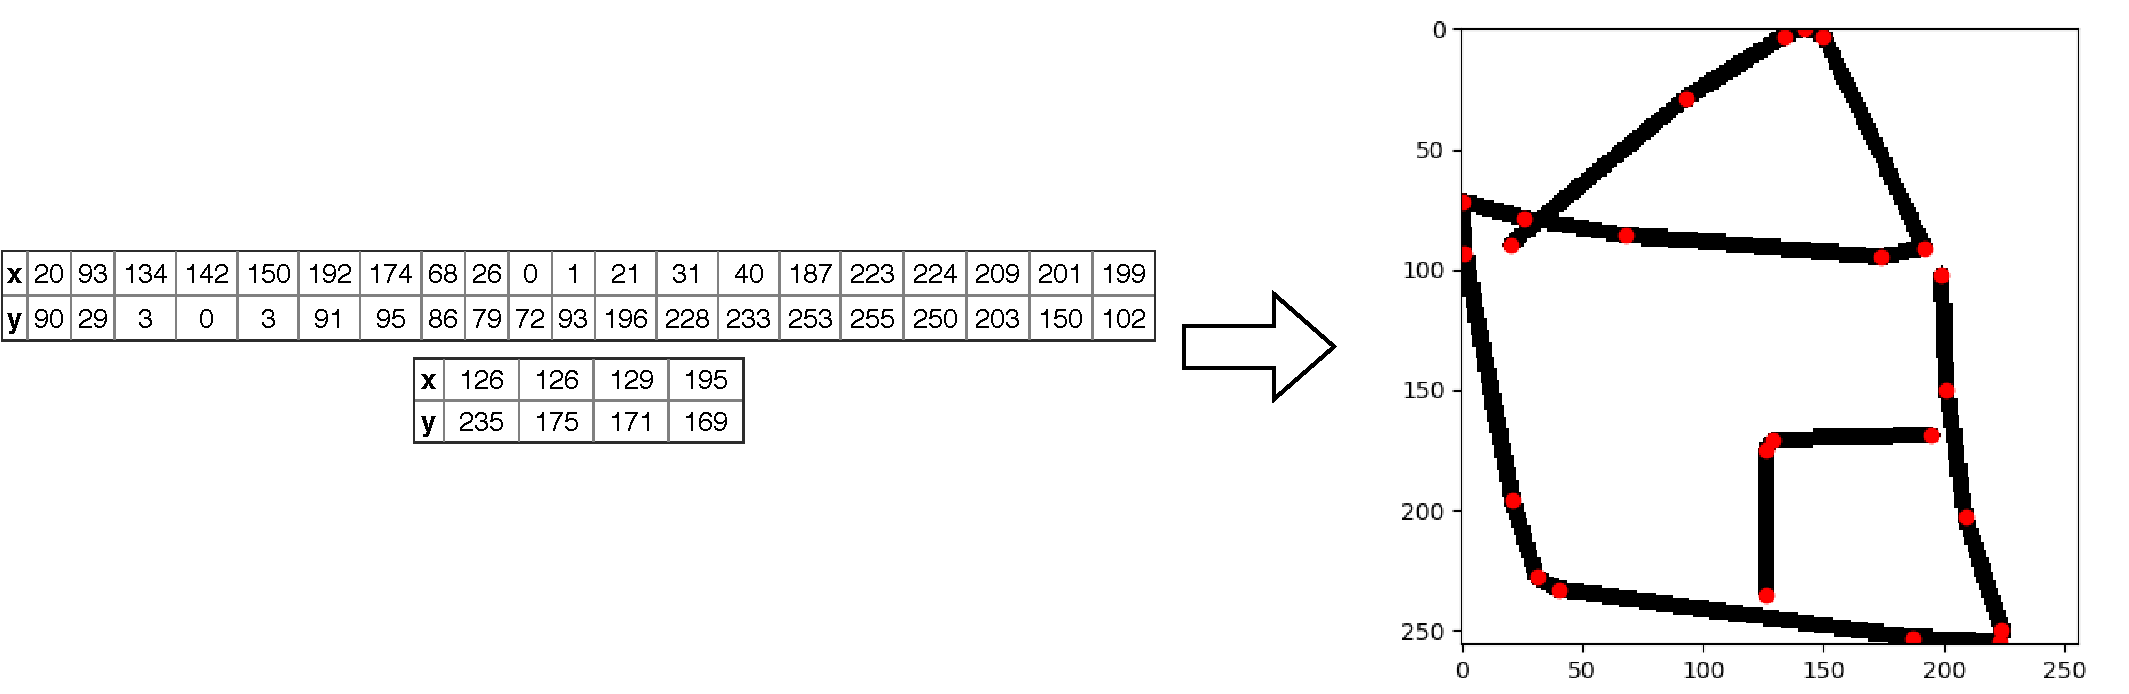
\includegraphics[width=\linewidth]{images/Transformations_horizontal.pdf} % Figure image
	\caption{Transformation de vecteur à image} % Figure caption
	\label{transformationimage} 
\end{figure}

On passe donc d'une série de positions en format csv à une image 256x256 à un seul canal en noir et blanc lorsqu'on vient charger les données dans notre modèle. Cette technique évite d'avoir à stocker toutes les données sous forme d'images qui occuperait probablement plusieurs GO qui seraient instockables avec nos ressources actuelles. 




La plupart des images sont loin d'être facile à apprendre pour un ordinateur, puisque que ces données ne sont pas filtrées par un humain qui peut valider si l'image est bonne. N'importe quel individu peut contribuer à cette base de données. Pour cette raison, on peut observer des images qui peuvent varier énormément pour une même classe. La figures \ref{frogs} nous permet de voir différentes images pour la classe \emph{frog}.



\begin{figure}[h]
	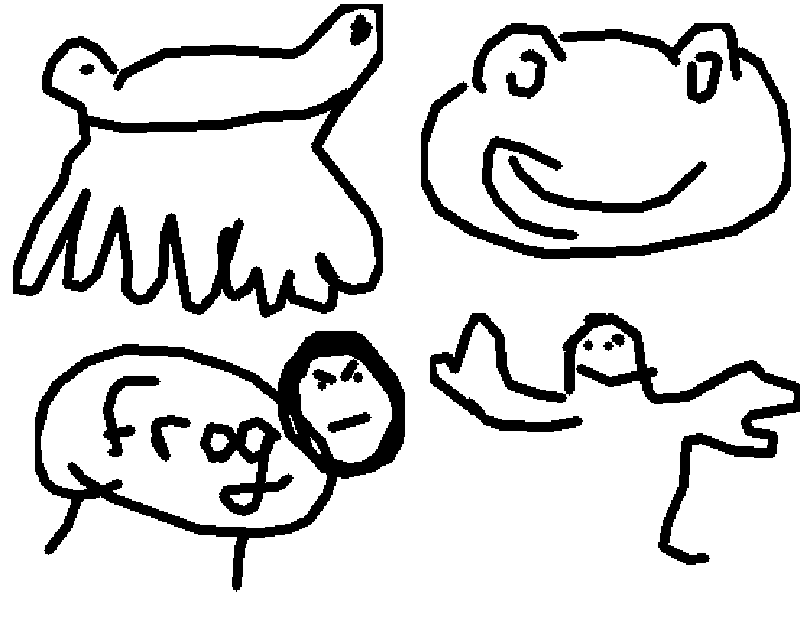
\includegraphics[width=\linewidth]{images/Combo_frogs.png} % Figure image
	\caption{Différentes images de la classe frog} % Figure caption
	\label{frogs} 
\end{figure}


On peut voir que les utilisateurs n'adoptent pas tous les mêmes techniques pour dessiner un même objet. Également puisque les utilisateurs ont seulement 20 secondes pour faire leur dessin, certains d'entre eux sont parfois incomplets. Comme aucun filtrage n'a été fait, on peut constater également que certaines images ne sont pas réalisés dans le but exact du projet (certains utilisateurs ne dessinent pas la bonne catégorie ou bien ne font qu'écrire le nom de la classe)


\section{Structure du modèle et méthodologie}
En gardant nos contraintes et enjeux en tête, il fallait trouver une façon efficace d'entraîner un modèle dans un temps raisonnable. Plusieurs techniques d'échantillonnage on pu être testées.


\subsection{Échantillonnage fixe par classe}

Le premier modèle testé est un modèle pré-entraîné avec architecture \emph{Resnet18}, mais avec un seul canal de couleur au lieu de 3. Pour entraîner le modèle, on procède d'une manière alternative étant donné qu'on ne peut pas se permettre de faire de vraies epochs complètes. 



Ainsi, à chacune de nos "epochs", on échantillonne (sans remise) un nombre $N$ fixe de données par classe parmi nos 150 000 données par classe. Ces $340N$ données servent à faire une "epoch"  pour notre modèle. On procède de la même façon à chaque "epoch" en ré-échantillonnant dans nos 150 000 données par classe (même celles pigées aux anciennes "epochs"). 
En entraînant de notre modèle de cette façon, il est possible que certaines données ne soient jamais vues et que d'autres le soient plusieurs fois.


Cette technique d'échantillonnage s'apparente au \emph{Bootstrapping} utilisé pour les méthodes par ensemble. Elle agit à la fois comme méthode d'échantillonnage aléatoire et comme méthode de régularisation. 
On peut s'attendre à ce que le modèle n'overfit pas excessivement notre jeu de données d'entraînement en procédant de cette façon puisque les données ne seront pas vues plusieurs fois de façon rapide et le réseau ne peut donc pas les apprendre par coeur.


Si on fait 35 epochs de la sorte avec un nombre $N=500$ (epoch de 170 000 données) on peut voir approximativement 11\% des données totales et environ 5.45\% des données vues sont échantillonnées plus d'une fois parmi les 35 epochs. 
On peut voir qu'on est assez loin de voir de voir la totalité du jeu de données même après les 35 epochs passées à cause de la quantité énorme de données disponibles. 
Toutefois, le modèle semble tout de même converger vers une précision de validation d'environ 76\% comme on peut le voir sur la figure \ref{histmodelnormal}. 
En utilisant un \emph{early stopping} et en utilisant les performances maximales sur le jeu de validation, on obtient une précision de validation de 77.44\%.


\begin{figure}[h]
	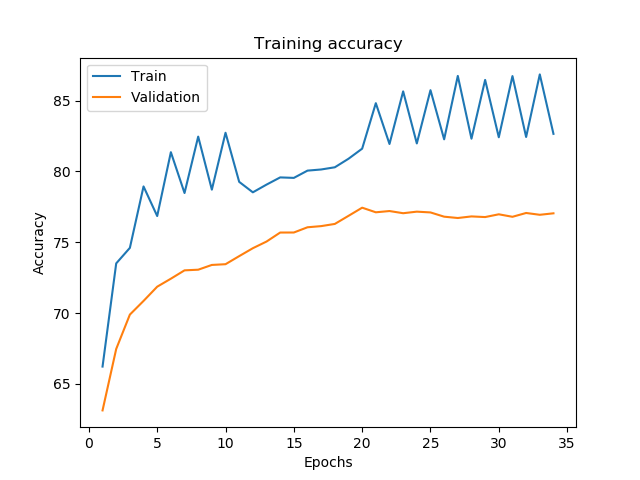
\includegraphics[width=\linewidth]{images/Model_general.png} % Figure image
	\caption{Historique d'entraînement avec entraînement standard} % Figure caption
	\label{histmodelnormal} 
\end{figure}


\subsection{Échantillonnage variable par classe}
La deuxième méthode d'entraînement est similaire à la première avec une légère modification qui essaie de privilégier les classes qui performment moins bien dans le but de simuler un processus de \emph{boosting}.


L'idée de base est d'échantillonner un plus grand nombre de données des classes qui sont mal prédites et un plus petit nombre pour celles qui sont bien prédites durant l'entraînement. 
À chaque epoch, on calcule notre précision par classe $A_i$ pour chacune des 340 classes. 
Pour effectuer notre epoch, on échantillonne $N_i$ données pour la classe i:

$$N_i=N(1-A_i)+0.25N$$
Où:
\begin{description}
\item[N]: Valeur constante pour toutes les classes (ex: 500)
\end{description}

Le terme $+0.25N$ permet de sélectionner au moins un minimum de données d'une classe qui performe déjà très bien pour que le modèle ne l'oublie pas lors la prochaine epoch.  Par exemple, on sélectionnerait $N$ données d'une classe avec 25\% de précision et $0.35N$ données d'une classe qui a 90\% de précision.


En appliquant cette technique d'apprentissage, on obtient une précision en validation de 79.53\% avec de l'early stopping. 
Cette technique d'échantillonnage ciblé nous permet d'aller chercher une précision supplémentaires d'environ 2\%.


\subsection{Modèle par ensemble avec couche de classification}
Le troisième modèle consiste à concaténer les sorties des 2 premiers modèles et à les passer dans une couche de classification linéaire. Pour l'entraînement de ce modèle, on gèle tous les paramètres des modèles \emph{Resnet18} et on entraîne seulement la couche de classification avec un échantillonnage fixe. La figure \ref{strutureensemble} illustre le processus.

\begin{figure}[h]
	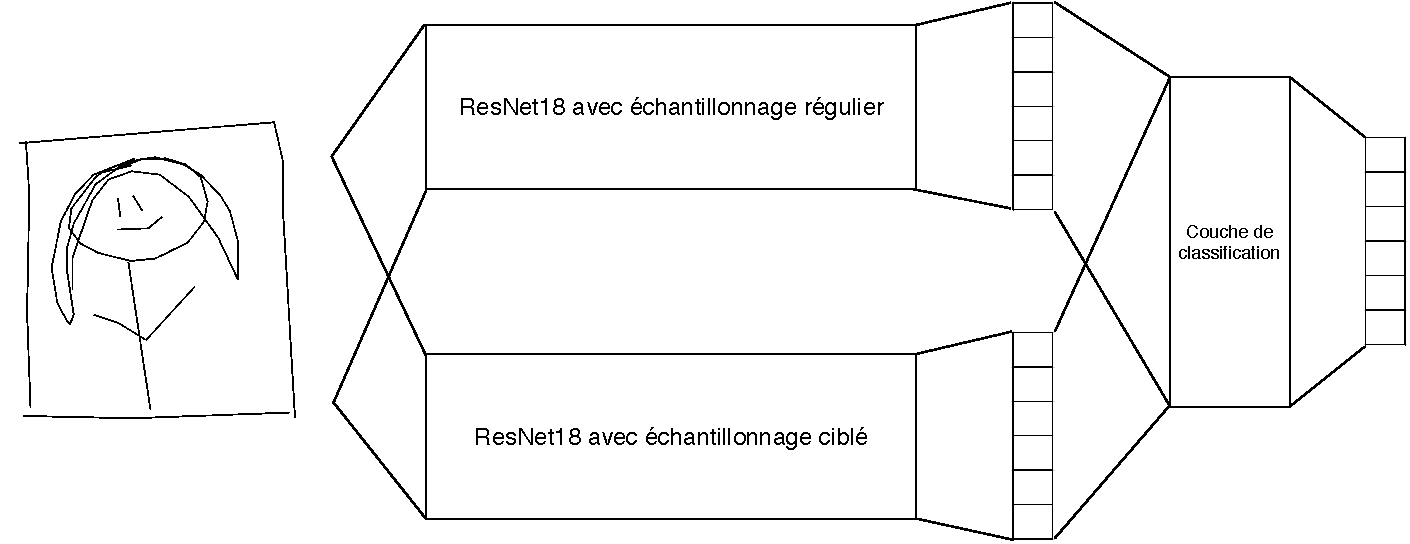
\includegraphics[width=\linewidth]{images/structure_reseau.pdf} % Figure image
	\caption{Modèle par ensemble avec couche de classification} % Figure caption
	\label{strutureensemble} 
\end{figure}


Par manque de temps, l'entraînement du modèle n'a pas pu être complété à 100\%, on peut toutefois voir l'historique d'entraînement du modèle sur la figure \ref{histmodelensemble}.


\begin{figure}[h]
	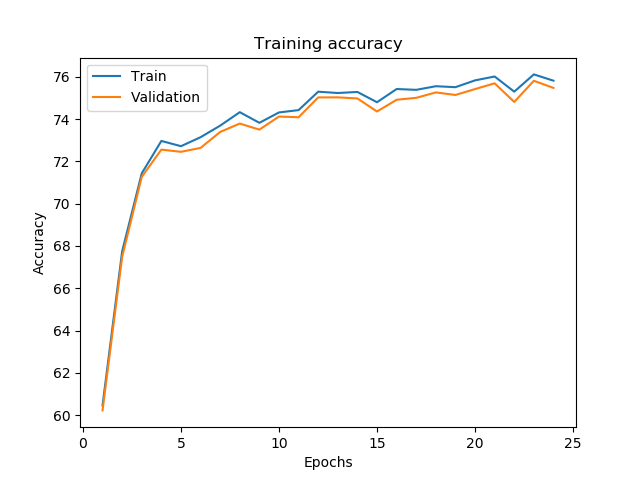
\includegraphics[width=\linewidth]{images/Model_ensemble.png} % Figure image
	\caption{Historique d'entraînement} % Figure caption
	\label{histmodelensemble} 
\end{figure}


On voit que la précision sur le jeu d'entraînement est pratiquement identique à celle de validation et qu'elles ne semblent pas encore avoir atteint un plateau lors de l'entraînement que ous avons fait. Il aurait été intéressant de voir les résultats après convergence puisque nous passons que cette technique aurait pu nous permettre d'obtenir des performances légèrement supérieures à notre deuxième modèle. 
Avec un \emph{early stopping}, on obtient une précision de 75.81\% en validation. 


\subsection{Modèle par ensemble avec moyenne simple des 2 premiers modèles}

Le dernier modèle que nous avons essayé est simplement d'utiliser la prédiction moyenne faite selon nos deux modèles \emph{ResNet18}. 
Cette technique par ensemble nous permet d'obtenir une précision de 79,94\% en validation, ce qui est légèrement supérieur à notre deuxième modèle entraîné avec échantillonnage ciblé. 




\section{Performances}
C'est l'intro 

das
d
as
da
sd
as
gsd
h
hhhhhhfghfgh tdh fgj fdj fg fg


\section{Conclusion}
C'est l'intro 

das
d
as
da
sd
as
gsd
h
hhhhhhfghfgh tdh fgj fdj fg fg



%----------------------------------------------------------------------------------------
%	BIBLIOGRAPHY
%----------------------------------------------------------------------------------------

\printbibliography[title={Bibliography}] % Print the bibliography, section title in curly brackets

%----------------------------------------------------------------------------------------

\end{document}
